

\documentclass[journal]{IEEEtran}

\usepackage{graphicx}
\usepackage{url}
\usepackage{cite}
\usepackage{authblk}
\usepackage[table,xcdraw]{xcolor}
\usepackage{amssymb}
\usepackage{amsmath}
\begin{document}


\title{An Investigation of Lossless Human Movement IMU Data Compression Methods}
% Compression of Kinematic Data
% Compression of Human Movement Data

\author[1]{David~Chiasson}
\author[1]{Junkai~Xu}
\author[1]{Peter~Shull}
\affil[1]{State Key Laboratory of Mechanical System and Vibration, School of Mechanical Engineering, Shanghai Jiao Tong University}

\maketitle

\begin{abstract}
Real-time kinematic data is central to many emerging technology applications, yet to date few techniques have been proposed to process and represent this relatively new information modality in an efficient manner. This paper explores techniques for the lossless compression of human kinematic IMU data. Techniques from traditional multimedia networks are compared with several novel approaches. Simple, computationally cheap techniques are shown to losslessly compress consumer-grade IMU kinematic data by a factor of ten to twenty, depending on movement activity, compared with traditional data representations. Furthermore, these simple techniques are shown to approach the optimal linear compression level. All techniques discussed in this study are implemented and released as open source C code using fixed point computation which can be integrated into a variety of computational platforms. 
\end{abstract}

\begin{IEEEkeywords}
kinematic data, human movement, compression, codec
\end{IEEEkeywords}



\section{Introduction}

\IEEEPARstart{M}{any} emerging technology applications rely on on real-time kinematic data as a crucial component. These applications include virtual reality, autonomous driving, internet of things, physical therapy, wearable electronics, and human performance among others. These applications have been enabled by the recent explosion of cheap inertial based sensors (IMUs) along with mobile computation power to process this data at high sampling frequency. Kinematic data represents a nascent field of multimedia data which is starkly under-developed compared to the existing maturity of text, audio, and visual type data processing techniques. In order to enable the modern applications listed above, efficient and standard techniques for representing and processing kinematic data are needed.

This study explores a range of both traditional and novel compression techniques applied to human kinematic data gathered by 6-axis IMUs. The best performing techniques are identified and discussed. Compression addresses two common problems present in modern human movement sensing applications: limited transmission bandwidth and limited storage space.

Only lossless compression techniques are considered in this study. The reason for this is that lossy compression inherently involves a value judgment about what information is useful and what information is irrelevant. In the absence of a specific application, no justification can be made for discarding any portion of information.

This study focuses on highly practical approaches which can be used in modern applications. To demonstrate this, all compression techniques have been implemented and released as open-source C code using fixed point computations. The hope of the authors is that this code can be a starting point for academic or industry developers implementing some kinematic data application on diverse computational platforms.

\begin{figure}
  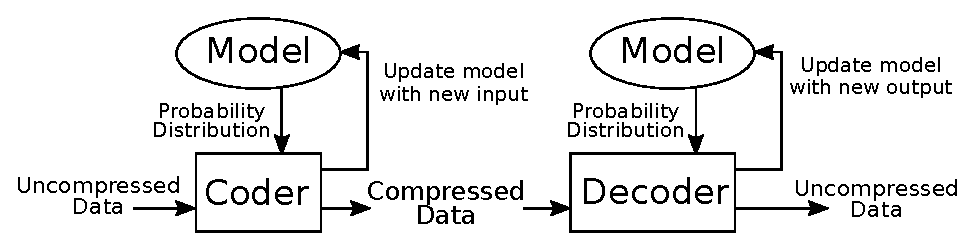
\includegraphics[width=\linewidth]{general_compressor.eps}
  \caption{General compressor and decompressor}
  \label{fig:general_compressor}
\end{figure}

A lossless compression algorithm can be divided into two components, modeling and coding as shown in figure \ref{fig:general_compressor}. The model incorporates prior knowledge about the signal to be compressed. It estimates a probability mass function (PMF) which represents the likelihood of all possible input symbols. A dynamic model is one which changes its PMF estimate after new input symbols are received. The Coder uses the PMF produced by the model to compute a unique variable length encoding for each possible symbol. Short encodings are assigned to likely symbols, and long encodings are assigned to unlikely symbols such that the total length of the compressed data is minimized. The decompressor uses an identical model to provide the same PMF to the decoder which is used to revert each code back into the original symbol. If the model is dynamic, this output is used to update the model for future predictions.

The coding component is well understood. The theoretical limit of coding performance on a signal with a know PMF is given by Shannon's noiseless coding theorem\cite{Shannon1948} as first order entropy:

$$H = -\sum_{i} P_ilog_2P_i$$

Furthermore, coding techniques have been developed which approach this limit under various conditions as early as 1952 \cite{Huffman1952}. Many near optimal techniques now exist with varying complexity and for various signal classes. Coding is thus considered a solved problem.

Modeling on the other hand must be revisited for each new signal class and application. Due to the pigeon hole principal, no algorithm can compress every possible input. Each model must make a implicit decision about the scope of signals that will be compressed. To the authors' knowledge, no previous work has directly addressed the modeling problem for kinematic data signals. This provides the motivation for the current work.

We hypothesize that compression ratios will be comparable to those achieved in lossless audio compression. We also hypothesize that the best performing codec will utilize some cross axis correlation and be informed by physics based models.

\section{Method}
For this study, the Human Gait Database (HuGaDB)\cite{Chereshnev2018} is used as a corpus to meaningfully and repeatable demonstrate the performance of various compression methods. HuGaDb is a public dataset of six-axis IMU signals collected from six different body segments of 18 healthy subjects performing 12 different movement activities sampled at 60Hz. This database was selected because it allows the comparison of compression techniques across body segment, subject, and activity in addition to sensor modality.

With the exception of traditional data representation techniques, all compression methods in this work will be presented as predictive models. The difference between the model prediction and observed sample will be referred to as the residual signal. All compression methods will encode this low entropy signal using Golomb-Rice coding to produce the final compressed data. Golomb-Rice coding is computationally efficient on binary base computational platforms, and has been shown to approach optimal coding if the input signal is geometrically distributed\cite{Golomb1966}\cite{F.Rice1979}.

\subsection{Traditional Methods}
In order to provide context for the performance of compression techniques, several traditional data representation formats are chosen as reference. In this study, the baseline data format (exhibiting a compression ratio of one) is comma separated value (CSV), a simple text based format which is the de-facto standard for storing sensor information. Performance of each compression technique is evaluated by computing the compression ratio CR relative to CSV via the following formula:
$$CR = \frac{\textrm{size of CSV file}}{\textrm{size of compressed file}}$$

In total, the following three traditional data representation formats were chosen to provide context for our results:

\begin{itemize}
  \item \textbf{CSV} Text based format considered the de facto standard. CSV files are ANSI encoded and formatted to have a constant length sample format to eliminate a source of randomness in our CR computation. Due to this decision, Binary format will have the same CR regardless of data properties. 
  \item \textbf{Binary} The optimal fixed size format. In our corpus, every sample is two bytes. This would be the optimal compression if each sample were an IID random variable uniformly distributed across the sample space.
  \item \textbf{ZIP compression of CSV} ZIP is a general purpose file compression format integrated into all major computer systems. ZIP was executed using the DEFLATE method \cite{Deutsch1996} and a compression level of 6.
\end{itemize}
\subsection{Tested Encodings}


Several restrictions are placed on the algorithms considered in this study. First, a viable algorithm must be causal. This is a basic requirement for an algorithm to be implemented in a real-time application. We also chose to only consider algorithms with zero filter delay. Since our sensors operate at a relatively low sampling frequency of 60Hz, a delay of one sample would be 16ms which is significant for modern information networks.

All algorithms considered in this paper are node independent. The model for each signal considers at most the information from the six co-located signals including it's own past input. While it is likely that utilizing inter-node correlation could produce better compression ratios, especially if a human biomechanics model is introduced, such an approach would limit the usefulness of said algorithm to a specific placement of nodes on the body.

Only lossless algorithms are considered. As discussed in the introduction, a lossy algorithm requires an objective metric for determining how much data loss and of what type is acceptable. Without this metric it is trivial to create a compression algorithm with an infinite compression ratio but which looses all information.

In practice, the implementation of a strictly lossless algorithm turns out to be non-trivial. This is because the standard for floating point computation IEEE 754 \cite{Society2008} is not sufficiently stringent to guarantee identical results on various implementations. For example, rounding of results may be slightly different between two computation platforms, or the same computation platform at two points in time. Additionally, a compiler or interpreter which processes the source code for an algorithm implementation will often utilize mathematical properties such as commutativity to optimize computation. This may result in different machines performing floating point operations in a different order which could lead to differing results even if each rounding operation were well defined by IEEE 754. In order to avoid both of these scenarios and guarantee identical results across diverse computational platforms, all algorithms in this study are implemented using integer operations and fixed-point 16.16 precision. There is significant cost associated with this technical decision. Namely that quantization error is independent of magnitude. This can lead to significant numerical issues for some algorithms.

The following lossless compression techniques are proposed in this study:
\begin{itemize}
  \item \textbf{Delta encoding} Current sample is predicted to be equivalent to the previous sample so that the difference between the two is encoded. If a signal varies slowly with time, this signal will be smaller than the original signal.
  \item \textbf{Linear extrapolation} Current sample is estimated as a linear extrapolation from previous samples. Also known as first order polynomial regression.
  \item \textbf{\boldmath$2^{nd}$ to \boldmath$5^{th}$ order polynomial regression} This technique assumes that the signal is a polynomial which is estimated from a least squares regression of past samples. This polynomial is then extended to get a prediction of the current sample.
  \item \textbf{Spline extrapolation} A spline is the minimum curvature piece-wise polynomial which connects a set of points. It is commonly used for interpolation, namely computer graphics smoothing. This technique was selected as splines are known to avoid Runge's phenomenon which is witnessed when extrapolating higher order polynomials. Results from the cubic spline with natural boundary conditions are presented in this paper.
\end{itemize}

\subsection{Optimal Model}

To complete the context for our proposed modeling techniques, we numerically compute the optimal linear model for our data. To do so, we will formulate our model as a linear prediction with the error, or residual signal defined as
$$\tilde{e} = Ax-b$$
Where each row of $A$ is the past history of our signal, each element of $b$ is the current sample, and $x$ is our model. For our application, we are interested in the residual signal which can be encoded into the minimum number of bits. To compute this, we consider the effect of Rice-Golomb coding on our residual signal. A Rice-Golomb encoding of order $M \in \mathbb{N}_0$, splits each $\tilde{e}_i$ into a quotient and remainder:
$$ q_i = \lfloor \frac{\tilde{e}_i}{2^M} \rfloor, r_i = \tilde{e}_i - q_i * 2^M  $$
The remainder $r_i$ is truncated binary encoded at a fixed size of $M$ bytes, while the quotient $q_i$ is unary encoded. The size in bits of each Rice-Golomb encoded element of the residual signal is thus:

$$ M + \lfloor\frac{\tilde{e}_i}{2^M}\rfloor + 1$$
If we relax our rounding operation, the size of each element can be approximated as a linear function of $\tilde{e}_i$ which leads to an approximate compressed size of:
 $$k+kM+ 2^{-M}\sum_{i=0}^k \tilde{e}_i$$
 Minimizing this value with $l$-1 normalization is equivalent to the optimization problem:
 
\begin{equation}
\begin{aligned}
& \underset{x}{\text{minimize}}
& & \left\Vert Ax-y \right\Vert_1 + \lambda\left\Vert x \right\Vert_1
\label{eq:optimize}
\end{aligned}
\end{equation}

$l$-1 normalization is used since it encourages sparsity in the model. Sparsity is desirable in this application as it reduces quantization error of the model coefficients and reduces the fixed point arithmetic error during execution. Both of these sources of error are significant when performing fixed point arithmetic. Since this problem is convex, it can readily be solved with a variety of numerical solvers. For this study, python bindings for the Splitting Conic Solver were used\cite{ocpb:16}\cite{scs}\cite{cvxpy}.

if problem \eqref{eq:optimize} is solved considering just past history, then the model for each axis of accelerometer and gyroscope can be computed independently. This model will be referred to as the optimal auto-correlation model. However, if we also take into account the past history of other axes and sensors, then the model can account for any cross-correlation which may result from the interrelated nature of rotation and orientation information. Solving problem \eqref{eq:optimize} with this expanded system will be referred to as the optimal cross-correlation model.

\subsection{Implementation}

To show algorithm performance in a realistic scenario, as well as to provide tools of benefit to the community, the algorithms in this study have been implemented in the C programming language and released as open-source code found at \url{https://github.com/dchiasson/kinetic_codec}. TODO[change the name of the repo, clean up docs, and release]. The choice of programming language as well as the restriction to integer arithmetic allow this code to be easily incorporated into programs executing on either a personal computer or embedded computation platforms, even those without a floating-point unit.

\section{Results}

Table \ref{table:all_stats} shows the CR of each compression method broken down by activity and body segment. All proposed compression methods outperformed traditional methods in size efficiency.

Delta encoding achieved the highest compression of the polynomial regression techniques (CR=12.75), and each higher degree polynomial performed progressively worse with 5th degree polynomial at the bottom (CR=11.25). The CR of delta encoding approached and occasionally exceeded that of the optimal auto- and cross-correlation model.

Low movement activities such as sitting and standing were compressed much more than high movement activities such as running (Fig:\ref{fig:movements}). Body segments showed little variation in CR although thigh locations showing slightly higher compression (Fig:\ref{fig:segments}).

\begin{figure}

  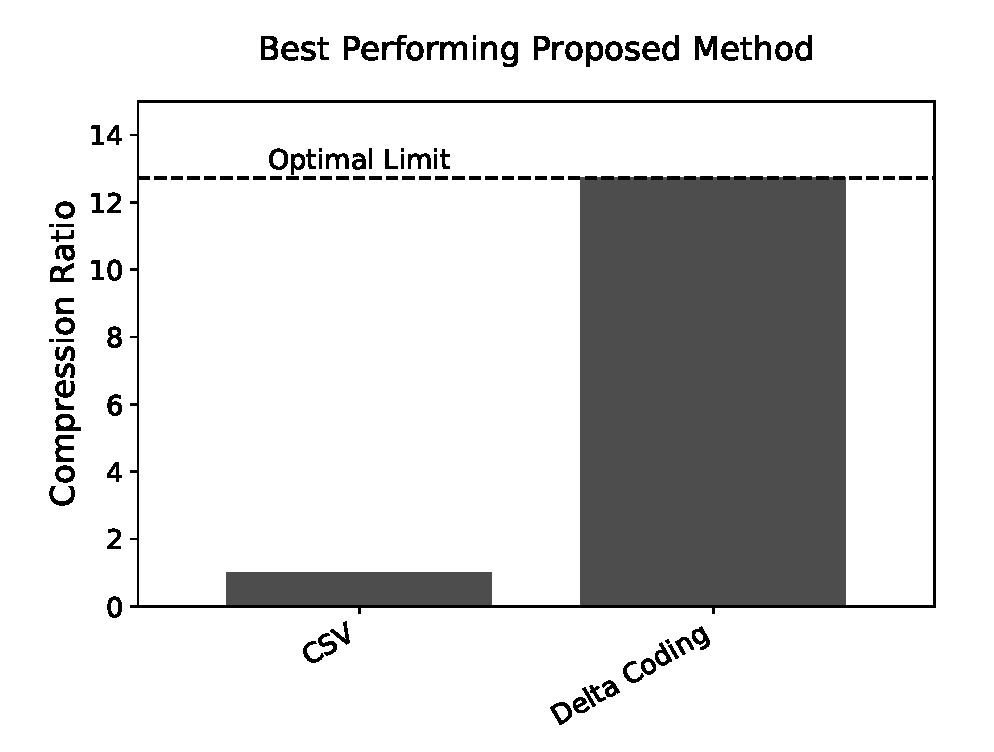
\includegraphics[width=\linewidth]{diff.eps}
  \caption{Compression ratio (original size / compressed size) of delta encoding compared with traditional CSV and the optimal auto-correlation model. Larger is better.}
  \label{fig:main_results}
  
\end{figure}
\begin{figure}

  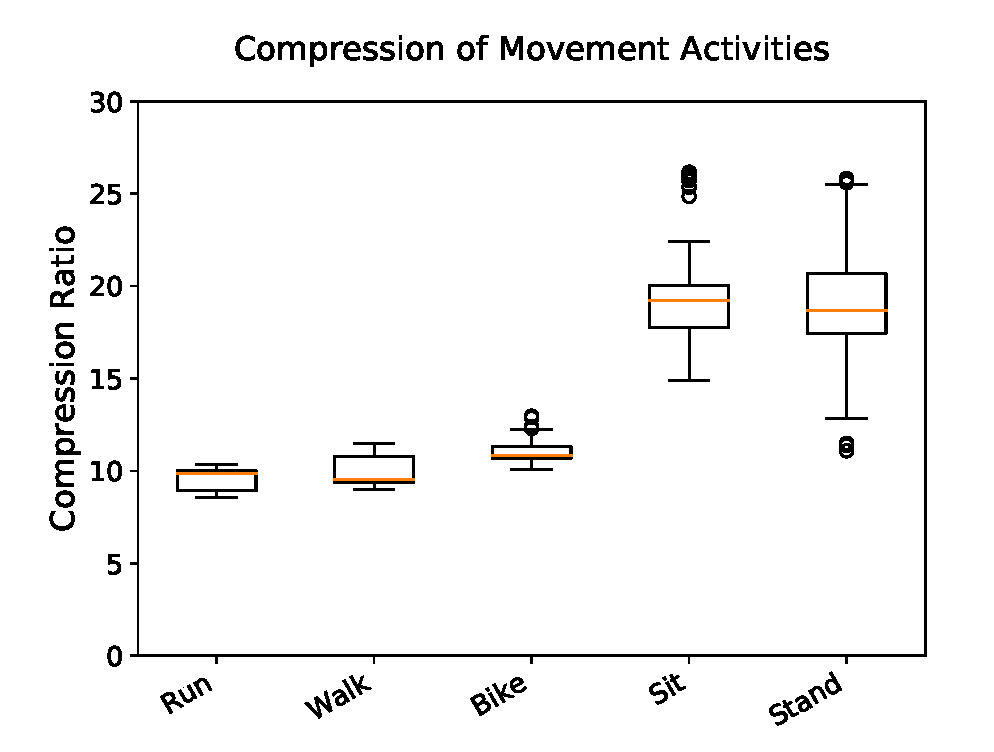
\includegraphics[width=\linewidth]{movement.eps}
  \caption{Compression ratio (original size / compressed size) of each movement activity using delta encoding. Larger is better.}
  \label{fig:movements}
  
\end{figure}
\begin{figure}

  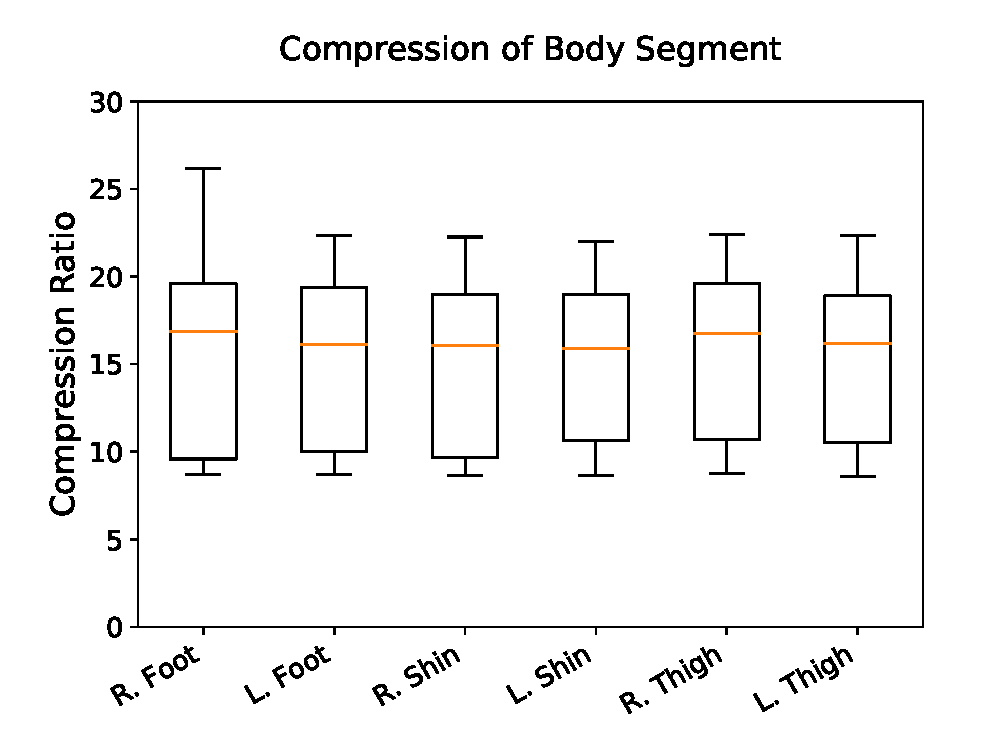
\includegraphics[width=\linewidth]{segment.eps}
  \caption{Compression ratio (original size / compressed size) of each body segment using delta encoding. Larger is better.}
  \label{fig:segments}
  
\end{figure}

%http://www.tablesgenerator.com/latex_tables
%http://calc2latex.sourceforge.net/

\begin{table*}[htbp]
\caption{Compression ratios for all methods across movement activity and body segment}
\label{table:all_stats}
\resizebox{\textwidth}{!}{%
\begin{tabular}{|l|r|r|r|r|r|r|r|r|r|r|r|r|}

\hline
 & \multicolumn{1}{l|}{\textbf{}} & \multicolumn{ 5}{c|}{\textbf{Activity}} & \multicolumn{ 6}{c|}{\textbf{Body Segment}} \\ \hline
 & \multicolumn{1}{l|}{\textbf{}} & \multicolumn{1}{l|}{\textbf{}} & \multicolumn{1}{l|}{\textbf{}} & \multicolumn{1}{l|}{\textbf{}} & \multicolumn{1}{l|}{\textbf{}} & \multicolumn{1}{l|}{\textbf{}} & \multicolumn{ 2}{c|}{\textbf{Foot}} & \multicolumn{ 2}{c|}{\textbf{Shin}} & \multicolumn{ 2}{c|}{\textbf{Thigh}} \\ \hline
 & \multicolumn{1}{l|}{\textbf{All}} & \multicolumn{1}{l|}{\textbf{Walk}} & \multicolumn{1}{l|}{\textbf{Run}} & \multicolumn{1}{l|}{\textbf{Sit}} & \multicolumn{1}{l|}{\textbf{Stand}} & \multicolumn{1}{l|}{\textbf{Bike}} & \multicolumn{1}{l|}{\textbf{R}} & \multicolumn{1}{l|}{\textbf{L}} & \multicolumn{1}{l|}{\textbf{R}} & \multicolumn{1}{l|}{\textbf{L}} & \multicolumn{1}{l|}{\textbf{R}} & \multicolumn{1}{l|}{\textbf{L}} \\ \hline
\textbf{CSV} & 1.00 & 1.00 & 1.00 & 1.00 & 1.00 & 1.00 & 1.00 & 1.00 & 1.00 & 1.00 & 1.00 & 1.00 \\ \hline
\textbf{ZIP} & 3.97 & 3.06 & 3.26 & 6.07 & 6.18 & 3.09 & 3.99 & 4.10 & 3.95 & 3.98 & 3.98 & 3.93 \\ \hline
\textbf{Binary} & 8.32 & 8.32 & 8.32 & 8.32 & 8.32 & 8.32 & 8.32 & 8.32 & 8.32 & 8.32 & 8.32 & 8.32 \\ \hline
\textbf{Spline} & 12.20 & 9.63 & 9.23 & 16.61 & 17.24 & 10.74 & 12.04 & 11.99 & 11.98 & 12.12 & 12.60 & 12.48 \\ \hline
\textbf{5th deg. poly.} & 11.25 & 8.92 & 8.59 & 15.28 & 15.78 & 9.87 & 11.24 & 11.16 & 11.10 & 11.20 & 11.49 & 11.34 \\ \hline
\textbf{4th deg. poly.} & 11.57 & 9.09 & 8.73 & 15.93 & 16.39 & 10.15 & 11.54 & 11.47 & 11.42 & 11.54 & 11.81 & 11.65 \\ \hline
\textbf{3rd deg. poly.} & 11.80 & 9.22 & 8.84 & 16.44 & 16.80 & 10.30 & 11.74 & 11.67 & 11.66 & 11.78 & 12.05 & 11.88 \\ \hline
\textbf{2nd deg. poly.} & 12.00 & 9.35 & 8.97 & 16.77 & 17.29 & 10.44 & 11.95 & 11.87 & 11.85 & 12.00 & 12.25 & 12.07 \\ \hline
\textbf{Linear} & 12.22 & 9.52 & 9.11 & 17.19 & 17.81 & 10.52 & 12.21 & 12.11 & 12.07 & 12.20 & 12.45 & 12.26 \\ \hline
\textbf{Delta} & 12.75 & 9.95 & 9.52 & 17.87 & 18.69 & 10.96 & 12.68 & 12.61 & 12.54 & 12.71 & 13.07 & 12.87 \\ \hline
\textbf{Optimal Auto} & 12.73 & 9.93 & 9.54 & 17.87 & 18.76 & 11.12 & 12.61 & 12.55 & 12.48 & 12.68 & 13.12 & 12.92 \\ \hline
\textbf{Optimal Cross} & 12.72 & 9.93 & 9.56 & 17.83 & 18.67 & 11.12 & 12.50 & 12.26 & 12.34 & 12.60 & 12.90 & 12.70 \\ \hline


\end{tabular}%
}%

\end{table*}



\section{Discussion}

These results show that even simple techniques result in a significant compression over the traditional encoding of CSV. If bandwidth or storage space is a concern in a kinematic data application then using any of the proposed methods would be an improvement.

Delta encoding performed surprisingly well, even exceeding that of the optimal linear models on several occasions. In theory, the optimal linear models should perform as good or better than delta encoding, since delta encoding was within the class of models that were optimized over in equation \eqref{eq:optimize} . The occasional inferior performance of the optimal linear models can be attributed to quantization error of the model coefficients and increase fixed point error from additional computational complexity. This explanation is supported by the observation that the cross-correlation model, which has a more complex model, often underperforms relative to the auto-correlation model while the opposite should be true in the absence of numeric error. Investigation of the optimal models' coefficients showed that they were similar to those of delta encoding.

The compression level achieved on each movement activity (Fig:\ref{fig:movements}) varied greatly, and appears roughly correlated with the intensity of movement involved in that activity. This matches our expectations as intuitively higher intensity of movement will have more information content. The compression of body segment information (Fig:\ref{fig:segments}) showed very minor variations save for slightly more compression of the thigh information. Intuitively, the thigh will experience less intense movement during most human movement. We can also observe minor differences between the compression of right and left body segments of the same type. Since the movement activities explored in this study are symmetric, these differences in compression are likely indicative of noise and bias differences between hardware sensors.

The similar performance of the cross-correlation optimal model and the auto-correlation optimal model does not support the expectation redundancy between accelerometer and gyroscope information. If such a linear correlation exists, it is too small to be usable in this practical application. This study does not preclude the possibility of a non-linear model to successfully exploit such a relationship.

\subsection{limitations}

The compression ratios presented in this paper are intended to demonstrate the relative difference between compression techniques and may not be representative of the absolute CR experienced in other applications. There are many other factors which can affect the compression ratio which are not explored in this paper. Namely, sensor differences of precision, noise, bias, and sampling rate are expected to have a large impact on the CR achieved. That being said, low-cost consumer grade IMUs were used for this study at a low sampling rate, and the authors would expect many applications to experience significantly higher compression than presented here if higher sampling rate or higher quality sensors are used.

The corpus chosen for demonstrating performance in this work allowed us to explore the effect of movement activity and body segment on compression. However, it could be improved for this purpose by including diverse hardware and higher sampling rates which would be more representative of applications.

In the future, the authors intend to expand these methods to include techniques for dynamic Rice K parameter detection and data packet drop recovery. Similar techniques can be readily borrowed from other mature multimedia fields.

\section{Conclusion}
This work explores methods for the compression of human movement kinematic data gathered from IMUs. Improved compression techniques can improve data transmission throughput and storage efficiency, potentially enabling new technology applications which were previously infeasible. For the corpus selected, delta encoding provided near-optimal linear compression (factor of 10-20 times) with very low computational cost.

\section*{Acknowledgment}
This work was supported by the National Natural Science
Foundation of China (51875347).

\bibliography{mendeley_citations,other_citations}{}
\bibliographystyle{plain}
%TODO: Make sure bib style is correct!
%\bibitem{IEEEhowto:kopka}

\clearpage
\section*{Scratch Section}
TODO: rewrite paragraphs below, maybe drop or move to method

The goal of the model is to produce an accurate PMF with minimum entropy. Intuitively this means that compression is higher the more "sure" the model is about some occurrences over other ones. If an optimal encoder is used, the compression ratio can be regarded as a quantitative measurement of the model's understanding of the underlying signal. Because of this, we expect the performance of various signal models to give us insight into the content of the kinematic signal.

The same coder and decoder is employed by all compression techniques explored in this work, and techniques are thus identified by the model used. Models are presented as predictive algorithms. Using this paradigm, the residual is the difference between each input symbol and what the model predicted the symbol to be. The compressed size is the first order entropy of the residual signal.


Consider deleting below:

TODO: why do we assume our signal is geometrically distributed about the mean!?
TODO: relationship for natural signals of residual signal and compression ratio

In this work, the maximum likelihood occurrence according to the model will be referred to as the prediction. The difference between the prediction and the actual sample will be referred to as the residual. For practical implementation, it is advantageous to convert the original signal into the residual signal before coding so that the coder can be computationally optimized to compute encodings for zero mean random variables (or same distribution? not recalculating ).

Define stream? node? anything else?

Linearized rotating gravity - A Newtonian physics based model in which a constant magnitude acceleration vector rotates according to gyroscope readings.

Finally, this study only explores linear models. Why is that?

 In the context of compression, complex or numerically unstable algorithms may produce compression ratios which underestimate their understanding of the underlying signal since their implementation is not equivalent to their mathematical derivation.

TODO: handle negatives in optimal filter derivation!

TODO: quantify statistical significance

Tables of detailed results k, order: total, accel/gryo, activity, segment, subject 

TODO: Discussion of cross stream FIR coefficients, pole zero plots, precision effect

TODO: Medical names for body parts?

TODO: can I prove that the optimal IIR linear filter cannot exceed that of the optimal FIR linear filter?

TODO: add algorithm execution time

TODO: Too many synonyms? [signal, data, file] [encoding, algorithm, model, technique, representation, compression, method]
TODO: audio compression comparison of methods and performance
TODO: what verb tense where?
TODO: demonstrate long implementation of compression technique to show that error is from quantization and fixed point error

\end{document}
